\documentclass[letterpaper,11pt]{article}
\title{CS475 Machine Learning, Fall 2012: Homework 5}
\date{}
\author{\bf Daniel Crankshaw dcranks1}


\usepackage[margin=1in]{geometry}
% \usepackage{hyperref}
\usepackage[colorlinks]{hyperref}
\usepackage{capt-of}
\usepackage{amssymb}
\usepackage{amsmath}
\usepackage{url}
\usepackage{graphicx}
\usepackage{color}
\usepackage{bbm}
\usepackage{float}
\usepackage{graphicx}
\usepackage{wrapfig}
\usepackage{url}
\usepackage{wrapfig}
\usepackage{hyperref} 
\usepackage{color}
\usepackage{amstext}
\usepackage{enumerate}
\usepackage{amsmath,bm}
\usepackage{fullpage}
    
\renewcommand{\baselinestretch}{1.15}    

\begin{document}

\maketitle

\paragraph{Question 1:}
\begin{enumerate}[(a)]
\item
\begin{equation}
V_c = (2r)^d
\end{equation}
\begin{equation}
V_s = \frac{r^d \sqrt{\pi}^d}{\Gamma (\frac{d}{2} + 1)}
\end{equation}
\begin{align}
\lim_{d \rightarrow \infty} \frac{V_s}{V_c} 
& = \lim_{d \rightarrow \infty} \frac{r^d \sqrt{\pi}^d}{2^d r^d \Gamma (\frac{d}{2} + 1)} & \text{let $d = 2z$}\\
& = \lim_{z \rightarrow \infty} \frac{r^2z \sqrt{\pi}^2z}{2^2z r^2z \Gamma (z + 1)} \frac{\frac{1}{\sqrt{2 \pi z} e^{-z} z^z}}{\frac{1}{\sqrt{2 \pi z} e^{-z} z^z}}\\
& = \lim_{z \rightarrow \infty} \frac{\frac{\sqrt{\pi}^{2^z}}{\sqrt{2 \pi z}e^{-z} z^z 2^{2z}}}{\frac{\Gamma (z + 1)}{\sqrt{2 \pi z}e^{-z} z^z}}\\
& = \lim_{z \rightarrow \infty} \frac{\pi^{z -.5} e^z}{2^{2z +.5}{z^{z +.5}}}\\
& = 0
\end{align}
\item
    Let us look at the $\epsilon$ ball variant of KNN. We have some
    n dimensional cube that represents our total feature space. And we pick
    a radius $\epsilon$ for our ball so that it encompasses some small but existent
    portion of the dataset. In low dimensions this is feasible to do. But in higher
    dimensions, we see that even if we pick the maximum possible diameter - the length
    of a side of the cube - then the ratio of the volume of our hypersphere to our total
    feature space will approach 0 (the limit from part a). This means that in high dimensions
    the probability of finding examples near our test example to create a label from will
    be 0, making prediction impossible.
\end{enumerate}

\paragraph{Question 2:}
\begin{enumerate}[(a)]
\item The 1-NN classifier will be $O(n d)$ assuming that the examples are not organized in
    a K-D tree. The linear SVM in primal form will be $O(d)$.
\item
    We should choose $K_2$. The $K_2$ classifier will have less variance than
    $K_1$ because it is less dependent on the training examples, but still has
    similar prediction power to the $K_1$ classifier becuase they achieve the
    same cross validation error.
\item
    KNN essentially draws boundaries between clusters. If the clusters are
    close together and dense, then KNN will have a hard time finding the
    right classification for examples on the border. In this case, a linear
    SVM on the K nearest neighbors will be helpful because it can distinguish
    that border no matter which side of the border the example we are trying
    to classify is on, as long as it can see examples on each side of the
    border. However, when we only have a few neighbors than the border that
    the KNN model learns will be very similar to the one that the linear
    SVM learns. This is because in sparser areas, the KNN algorithm works
    much better and is less sensitive to small changes in the location of
    the example, and so the linear SVM will learn a similar boundary.
\end{enumerate}

\paragraph{Question 3:}
\begin{enumerate}[(a)]
\item
    In this case, we make the observation that the condition is satisfied
if $x_1 - x_2 \leq 0$ and $1 \leq -x_1 -x_2 <= -1$. $T_0$ handles the first case
and $T_{-1}$ handles the second case. Each output -1 if activated, and so the
condition is only satisfied if both cases are satisfied.
\begin{figure}[H]
    \centering
    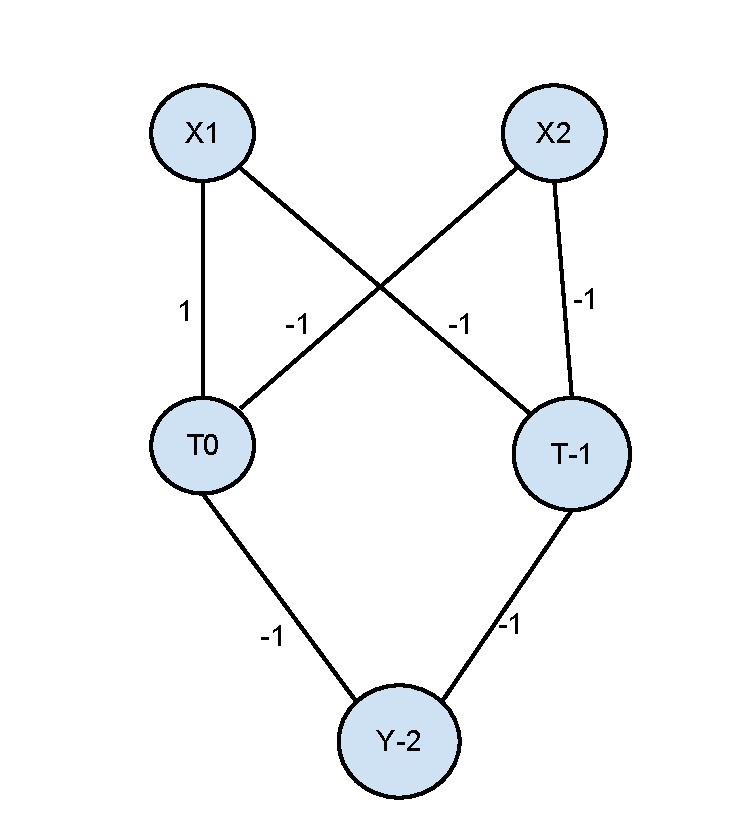
\includegraphics[scale=0.5]{hw5-3a.pdf}
\end{figure}
\item
    In this case we recognize that the shape we are recognizing is a square
    and so we must check that our point is within the square. We can decompose this
    into recognizing whether it is on the correct side of each of the four borders
    of the square. These conditions translate to $x_2 - x_1 \leq 1$,
    $x_2 + x_1 \leq 1$, $x_1 - x_2 \leq 1$ and $-x_2 - x_1 \leq 1$.
\begin{figure}[H]
    \centering
    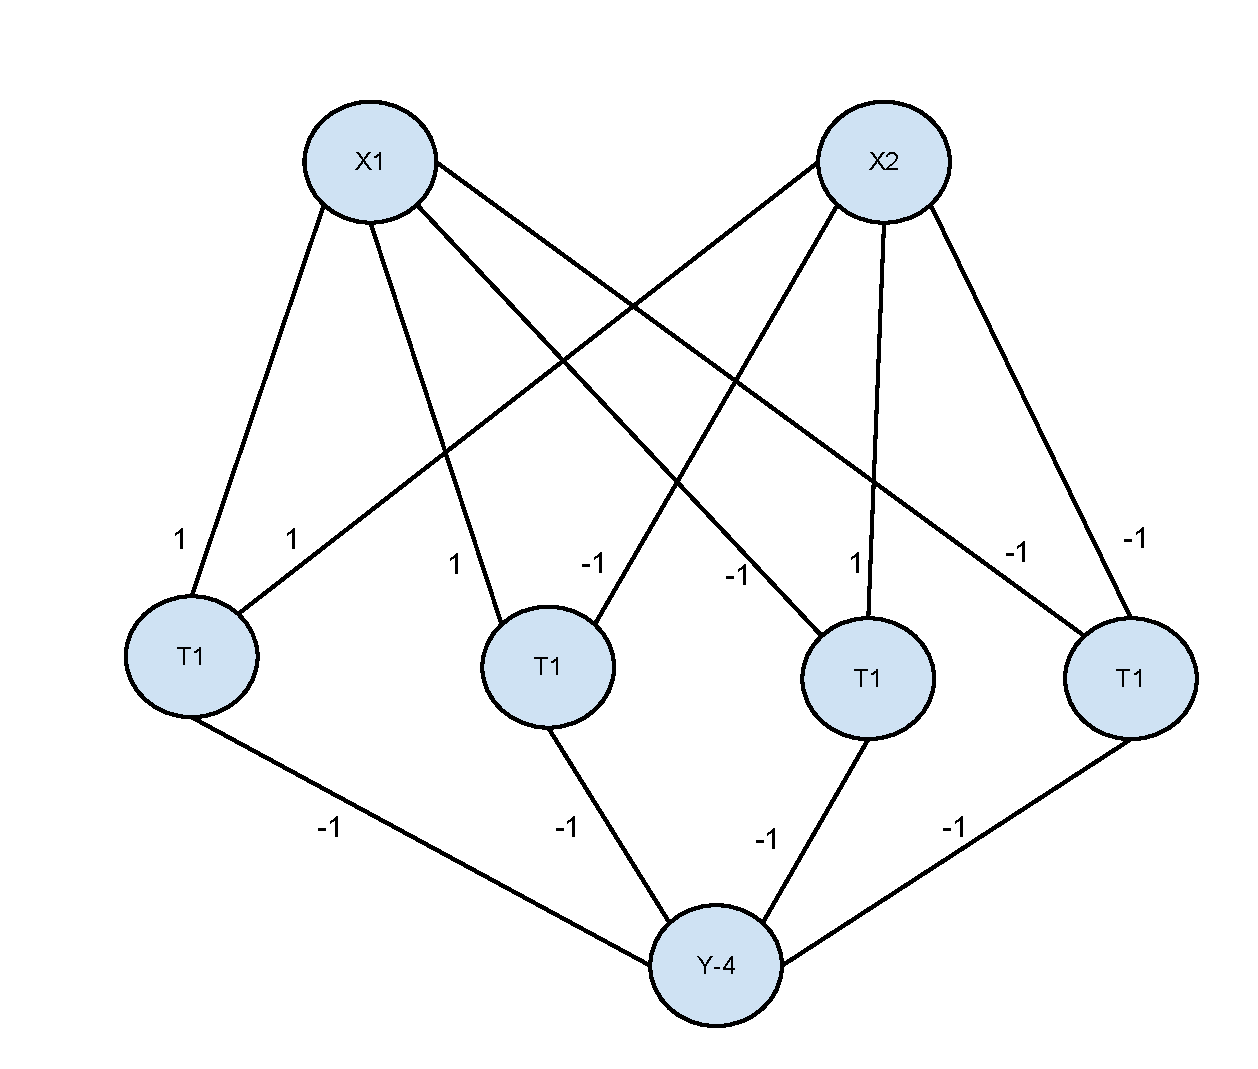
\includegraphics[scale=0.5]{hw5-3b.pdf}
\end{figure}
\item
    To approximate $x_1^2 + x_2^2 \leq 1$, we must figure out a way to approximate
    a circle. We can do this by approximating the circle with a many-sided polygon
    circumscribing it. Similarly to the square in the previous example, we
    can decompose this into a set of independent conditions that must be fulfilled
    (the point we are looking at must be on the right side of each bounding line).
    The more sides we add to the polygon, the better the approximation will be.
\end{enumerate}

\paragraph{Question 4:}
This method is exactly the same as the AdaBoost algorithm, as the additional
factor in the exponent will be cancelled out when adjusting the normaliziation
constant for the rounds probability distribution.

\end{document}

